
\documentclass[10pt,letter]{article}
	% basic article document class
	% use percent signs to make comments to yourself -- they will not show up.

\usepackage[letterpaper, margin=1.4in]{geometry}
\usepackage{amsmath}
\usepackage{amssymb}
\usepackage{amsthm}
\usepackage{mathtools}
\usepackage{dsfont}
	% packages that allow mathematical formatting
\usepackage[toc,page]{appendix}
\usepackage{graphicx}
	% package that allows you to include graphics

\usepackage{setspace}
	% package that allows you to change spacing
\usepackage{float}

\onehalfspacing
	% text become 1.5 spaced

\usepackage{fullpage}
	% package that specifies normal margins

\usepackage[document]{ragged2e}


%%%%% User-defined command %%%%%
% define floor and ceil
\newcommand{\floor}[1]{\lfloor #1 \rfloor}
\newcommand{\ceil}[1]{\lceil #1 \rceil}

%%%%% Title Page %%%%%
\title{\textbf{STA2202 Data Analysis Report}\\
\doublespacing
\large{A Forecast On DJIA Monthly Excess Return Of April 2017}}
\author{
  Suolawangzai\\
  \texttt{}
}
	
\begin{document}
	% line of code telling latex that your document is beginning
	\pagenumbering{gobble} 
	% Note: when you omit this command, the current dateis automatically included
 	\maketitle 
	% tells latex to follow your header (e.g., title, author) commands.
	\newpage
	\pagenumbering{arabic}
\section*{Abstract}
\paragraph{} After careful analysis and examination, we found that the ARMA(2,2) model fits the data on monthly excess return of Dow Jones Industrial Average from January 2005 to February 2017 best. Based on the ARMA(2,2) model, the monthly excess return of April, 2017 is predicted to be 0.00103822. The 95\% prediction interval for the estimation is (-0.07091359, 0.07299003).
\paragraph{} The graph below shows the monthly excess return data from January 2005 to February 2017 and its predicted values for March and April 2017 with 80\% and 95\% prediction intervals.\footnote[1]{Note that the x-axis representing time has been normalized, see details in following analysis.}
\begin{figure}[H]
    \centering
    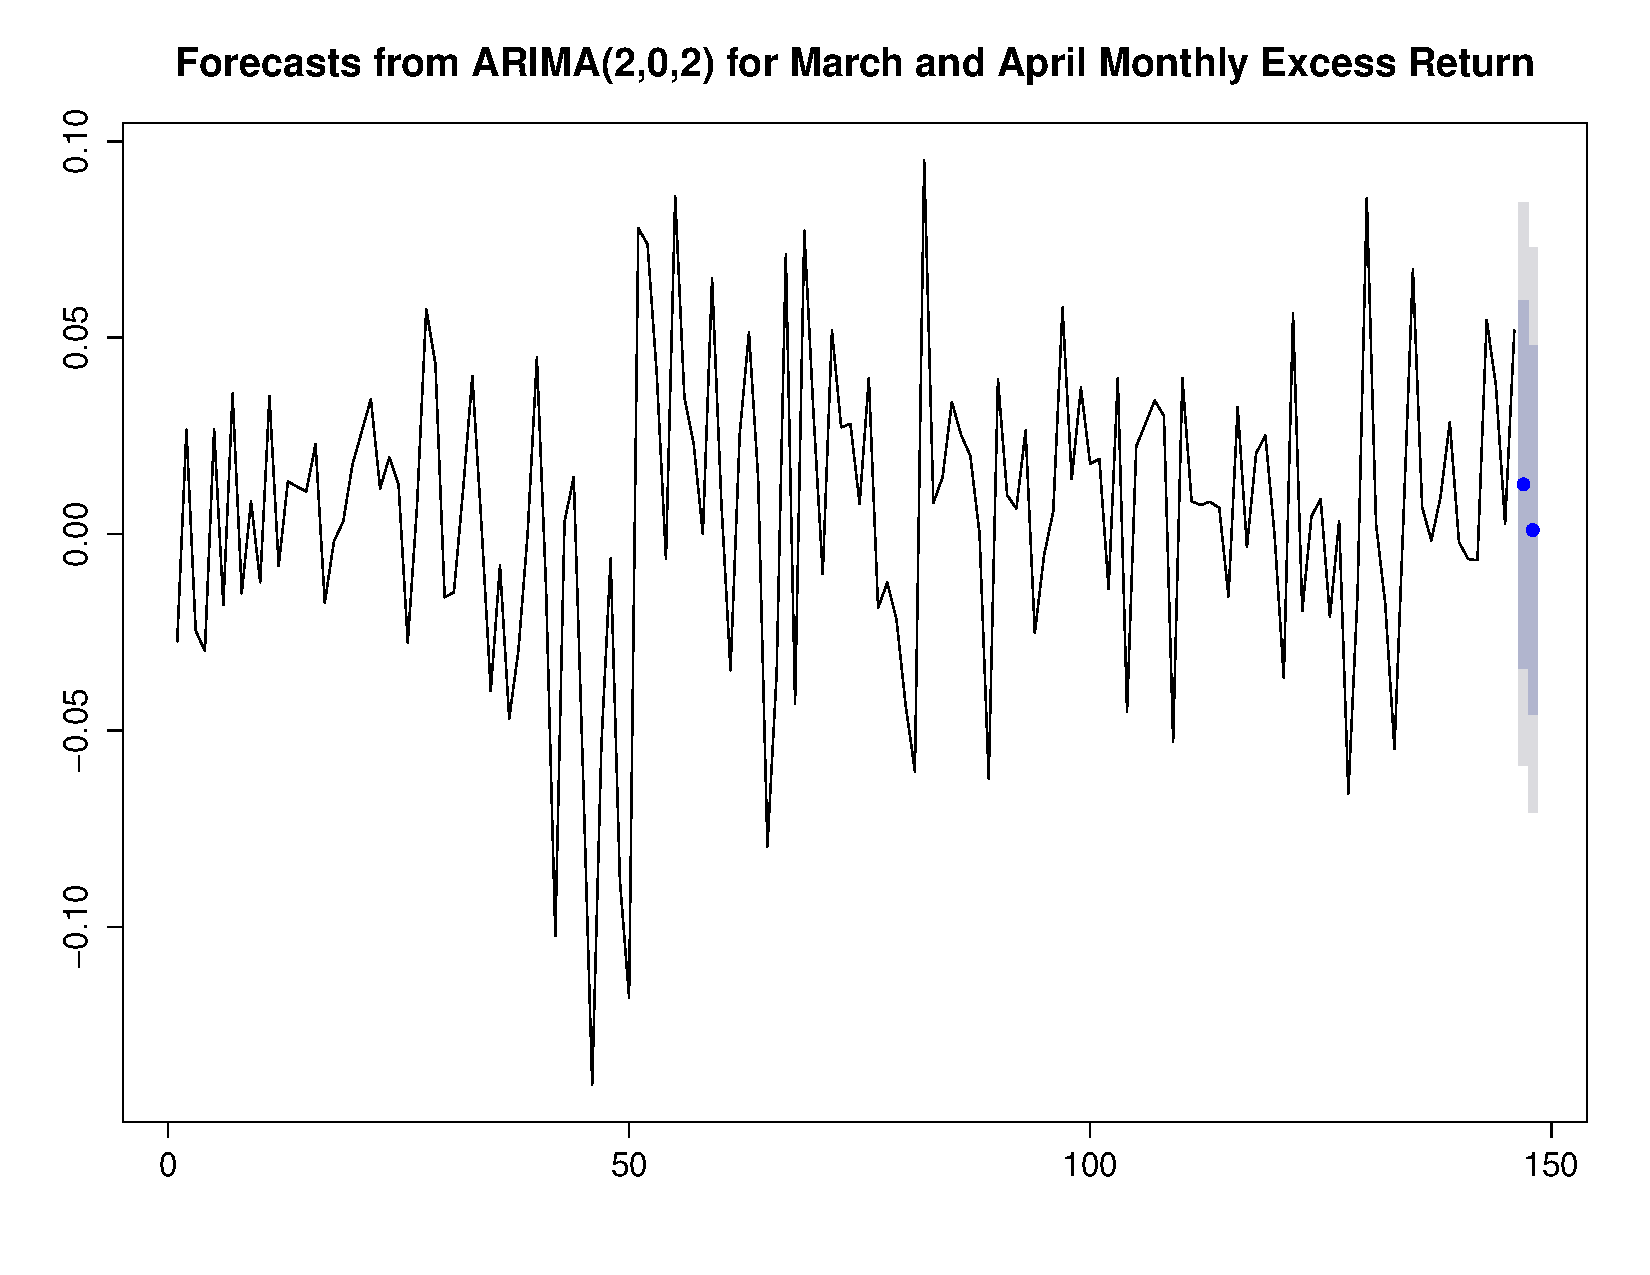
\includegraphics[width=0.8\textwidth]{/Users/zuoyuzhang/desktop/DataAnalysis/Forecast.pdf}
    \caption{Monthly excess return vs Time (with Prediction Values and Prediction Interval)}
    \label{fig}
\end{figure}
\section*{Data Acquisition}
\paragraph{}Through Yahoo finance \footnote[2]{The data is retrieved from https://ca.finance.yahoo.com/quote/\%5EDJI?ltr=1}, we retrieved the data on the open price of Dow Jones Industrial Average in each month from January 2005 to March 2017 \footnote[3]{The reason we included data of Mar 1st 2017 is to calculate the excess return of February 2017}. By applying the formula below, 
$$\text{Monthly excess return} = \frac{\text{Close price of the month} -\text{Open price of the month}}{\text{Open price of the month}}$$
we obtained the data on monthly excess return of 147 months from January 2005 to February 2017. For convenience, I relabelled the time series, so $t=1$ corresponds to January 2005, $t=2$ corresponds to February 2005 and so on. The remaining analysis is based on this relabelled time series. I'll use it to forecast the monthly excess return of April, 2017.
\section*{Preliminary Check}
\paragraph{} First, plot series of monthly excess return against the time index (see Figure 2 in Appendix). The monthly excess return is very volatile, but it seems there is no obvious trend and seasonality appearing. The monthly excess return appears only oscillate drastically around 0 over time, however, with no visible strong trend. It seems appropriate to fit a stationary and non-seasonal model to the time series.
\paragraph{} The observation is also confirmed by the autocorrelation plot of the date series (see Figure 3 in Appendix), the ACF function shows no pattern of periodicity. Hence, the time series need no seasonal adjustment. Additionally, the ACF of monthly excess return drops to zero rather quickly, with only two autocorrelations outside the 95\% confidence band, which suggests the stationarity of the data. If the time series is not stationary, its ACF will decrease rather slowly. To further test whether differencing is necessary for our data, we use the unit root test. We conducted the Augmented Dickey-Fuller (ADF) test\footnote[4]{In R the ADF test is conducted by suing function adf.test()} on our data with null-hypothesis being the data are non-stationary. We obtained a p-value that is much less than 0.05, indicating that the time series is indeed stationary as we thought. Therefore, we can fit a non-seasonal and stationary model to our data.

\section*{ARIMA Model}
\paragraph{} As discussed above, we can use a non-seasonal and stationary model to fit our data. According to correlogram (Figure 3 in Appendix) of the data, the ACF is significantly different from 0 at lag 0 and lag 4 and the ACF shows a pattern of decay, so it's unlikely that the data follows the white noise. To formally verify that, we conduct the Ljung-Box test\footnote[5]{In R the Ljung-Box test is conducted by using function Box.test()} on the time series and obtained a p-value of 0.00144 which is much less than 0.05, implying that the data is significantly different from the white noise process. Moreover, by using qq-plot (Figure 4 in Appendix), we can also rule out the possibility to use Gaussian model to fit the data, since we can see from the figure that the qq-plot of the data do not fit the straight line very well. 

\paragraph{}
As mentioned above, the ACF of data shows the pattern of decay overtime. There are significant spikes at lag 4 and 6 and beyond that all autocorrelations stay inside the 95\% confidence band. Similarly, for the PACF, there is a significant spike at lag 3 and all partial autocorrelations at lags greater than 3 lie within the confidence band. These observations from ACF and PACF plot suggest that a model with a MA process component and an AR process is suitable. Hence, it is reasonable to fit an ARMA model to the data.

\paragraph{} Since ARMA(p,q) is a suitable model for our time series, then next thing we did was to identify parameters p, q of the model. We used Akaike's Information Criterion corrected for bias (AICc) in selecting the best $q$ and $p$. Based on observations of significant spikes in ACF and PACF plots, it's reasonable to examine model with p ranging from 0 to 5 and q from 0 to 7. For each combination of (p,q), we used maximum likelihood method to fit each ARMA(p,q) model to the data and calculated every AICc. The best (p,q) is the one minimizes the AICc. After fitting 48 models, we picked three smallest AICcs, which are -541.5136 from ARMA(4,4), -540.5804 from ARMA(2,2) and -539.4145 from ARMA(3,3)\footnote[6]{Numbers are calculated using function arma() in package 'itrsm' in R}. By criterion, ARMA(4,4) seems to be the best model. However, as can been seen from numbers we obtained, the AICc only improved a little (i.e less then 1) from ARMA(2, 2), but the number of parameters increased by 2. Usually, the model with the fewest parameters is better. Since the improvement of AICcs are not large enough from ARMA(4,4) to ARMA(2,2), we concluded that ARMA(2,2) is the best model.  

\paragraph{} Since ARMA(p,q) model are special case of ARIMA(p,d,q) with $d=0$, we can directly search for the best model among ARIMA models. Therefore, in addition to analysis and calculation above, we also directly applied Hyndman-Khandakar algorithm \footnote[7]{The auto.arima() function in the 'forecast' package of R uses a variation of the Hyndman-Khandakar algorithm which combines unit root tests, minimization of the AICc and MLE to obtain an ARIMA model. The function conducts a search over possible model within the order constraints provided and returns best ARIMA model.} in our search for the best ARIMA(p,d,q) model based on AICc among models with p and q in the same range as we stated before, and d ranging from 0 to 2.  The best model fitting the data given by the algorithm is also ARIMA(2,0,2), which is the same as the ARMA(2,2). This result further justified the usage of ARMA(2,2) model to fit the data.

\paragraph{} Therefore, we used ARMA(2, 2) model to fit the monthly excess return data.

\section*{Diagnostic Examination}
\paragraph{} To further check the appropriateness of ARMA(2,2) model, we compare the observed values with the corresponding predicted values obtained from ARMA(2,2) model. If ARMA(2,2) is an appropriate model for data, then the residuals should behave like the white noise and normally distributed. 
\paragraph{} We first plotted the residuals against the time (see Figure 5 in Appendix). Note that the graph do resembles the plot of the white noise sequence, since there is no indication of non-zero mean or non-constant variance. Therefore, on this basis, there is no reason to doubt the appropriateness of the ARMA(2,2) model. Moreover, ACF and PACF plotted are also consistent with white noise series, with all autocorrelations and partial autocorrelations lying within the 95\% limits (see Figure 5 in Appendix). 

\paragraph{} To formally verifies that residuals are normally distributed white noise, we used Ljung-Box test again to test residuals of ARMA(2,2) model. The test returned a p-value of 0.8993, which is much greater than 0.05. With the null hypothesis stating that the residuals are random normally distributed, we cannot reject the null hypothesis. Additionally, the qq-plot of residuals is also consistent with our conclusion, since there is no obvious deviation from straight line in qq-plot (see Figure 6 in Appendix), there is no evidence to reject normality hypothesis.
\paragraph{} Since ARMA(2,2) passes all the diagnostic checks above, we conclude that ARMA(2,2) is indeed the best model. Next, we'll use it to forecast. 

\section*{Forecast}
\paragraph{} After ARMA(2,2) is fitted to data, we can use innovation algorithms to compute the best 2-step linear predictor and prediction errors recursively. In this report, we compare the results from two functions (i.e predict() and forecast() in R) that calculate the best linear forecast of the ARIMA model. The resulting predictions for the next two periods from predict() function are 0.012686983 and 0.001038629 respectively, while the results from forecast() function are 0.01268854 and 0.00103822. The answers are very similar. However, since forecast() function are more enhanced predicting function intended for time series model, we adopt the the latter results. Therefore, by our construction of the time series, the prediction for the monthly excess return in April 2017 is 0.00103822.  The prediction errors are also calculated together with the predictor recursively along the way, hence the interval prediction can also be constructed. The forecast() function also returns the 95\% prediction interval, which is $(-0.07091359, 0.07299003)$.

\paragraph{} They way we constructed forecast interval by using prediction errors involving two assumptions. One is that residuals are uncorrelated and normally distributed, the other is that the fitted model is in fact the true model for the data. As we demonstrated in diagnostic check section, the residuals of ARMA(2,2) are indeed uncorrelated and normally distributed. Hence, we can safely compute 95\% confidence interval for the estimation using normal distribution. With regard to second assumption, since we don't know the underlying true model, the variation of the prediction errors may be underestimated, because variation in the estimation of parameters is not included in the calculation\footnote[8]{In forecast() function, the standard errors of prediction exclude the uncertainty in the estimation of the ARMA model and the regression coefficients.}. However, if the sample size is large, the effect of errors in parameter estimation is negligible. Since our data on monthly excess return have 147 data points, we can neglect this effect. Therefore, interval ( -0.07091359, 0.07299003) we obtained is a valid prediction interval.

\clearpage
\appendix
\center
\title{\huge{\em{Appendix}}}
\begin{figure}[H]
    \centering
    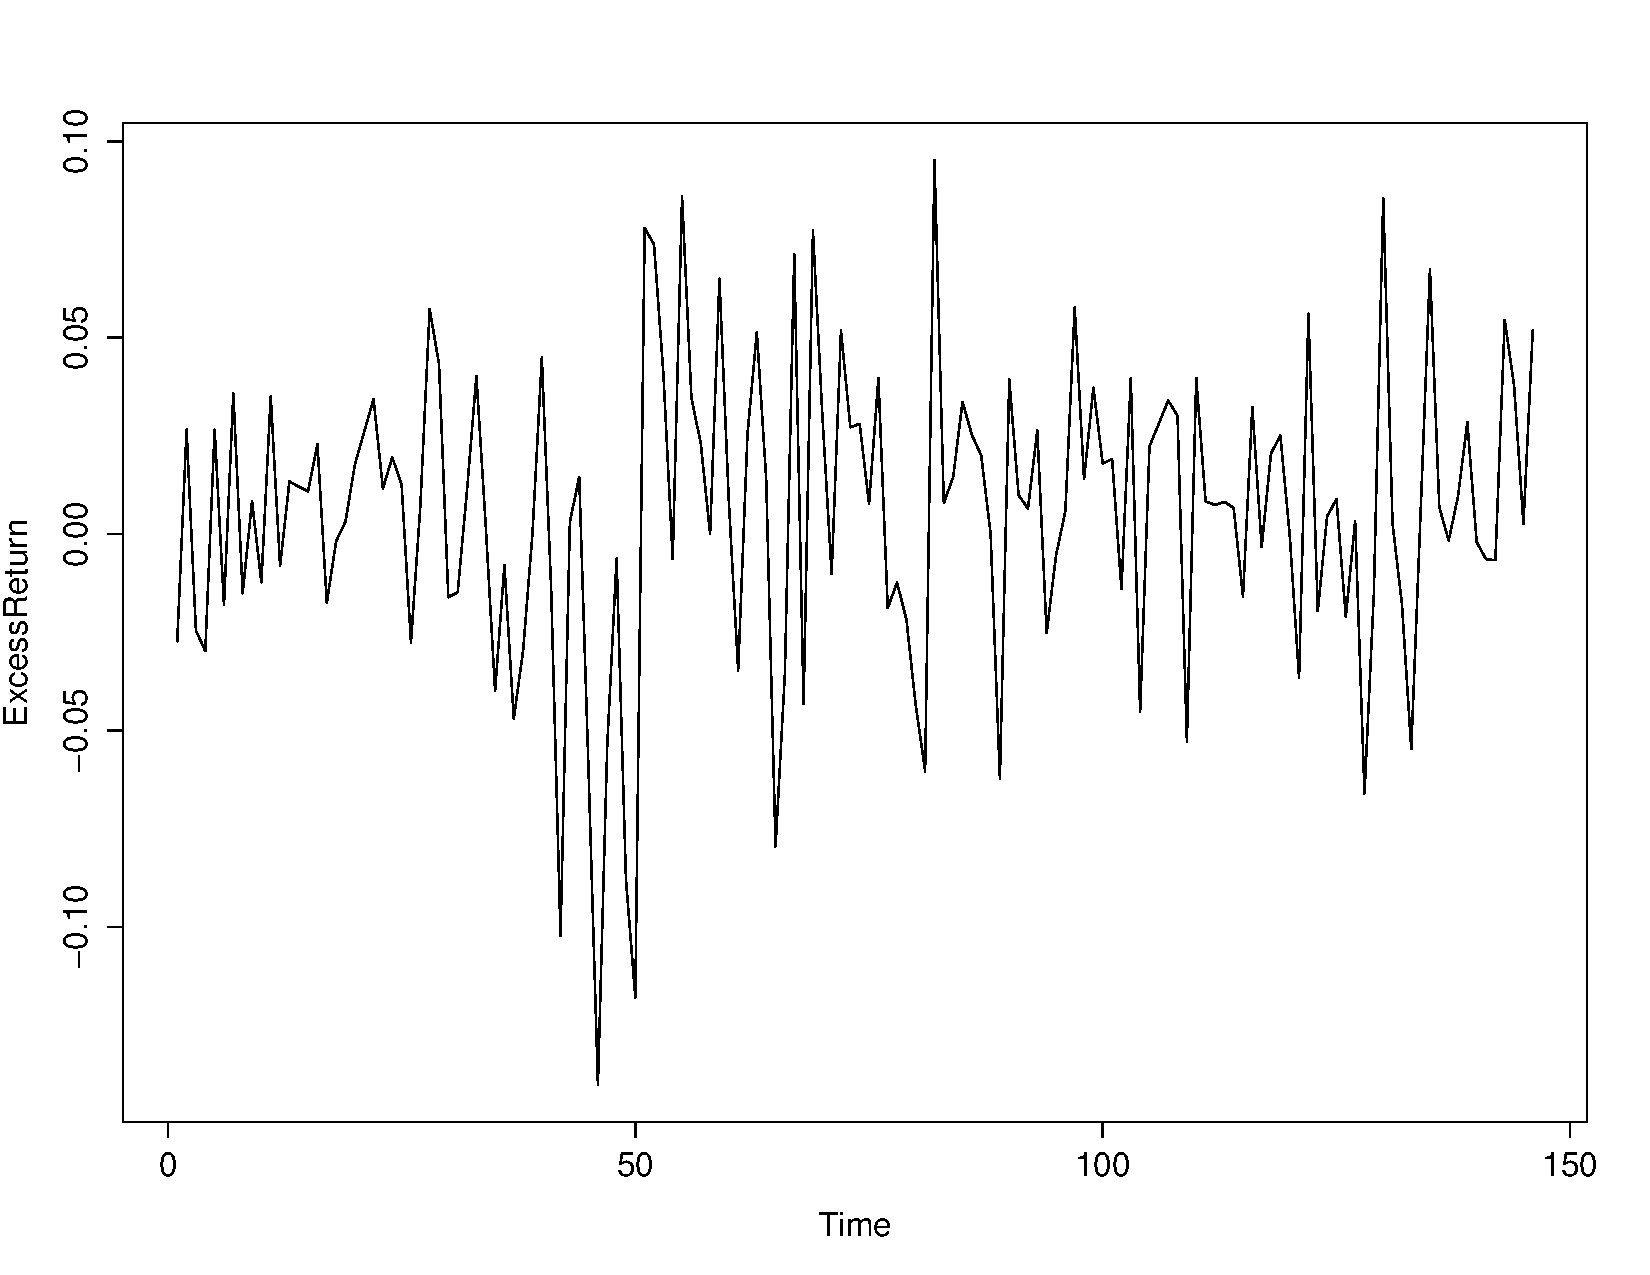
\includegraphics[width=0.8\textwidth]{/Users/zuoyuzhang/desktop/DataAnalysis/1TimeSeriesPlot.pdf}
    \caption{Monthly excess return vs Time}
    \label{fig}
\end{figure}

\begin{figure}[H]
    \centering
    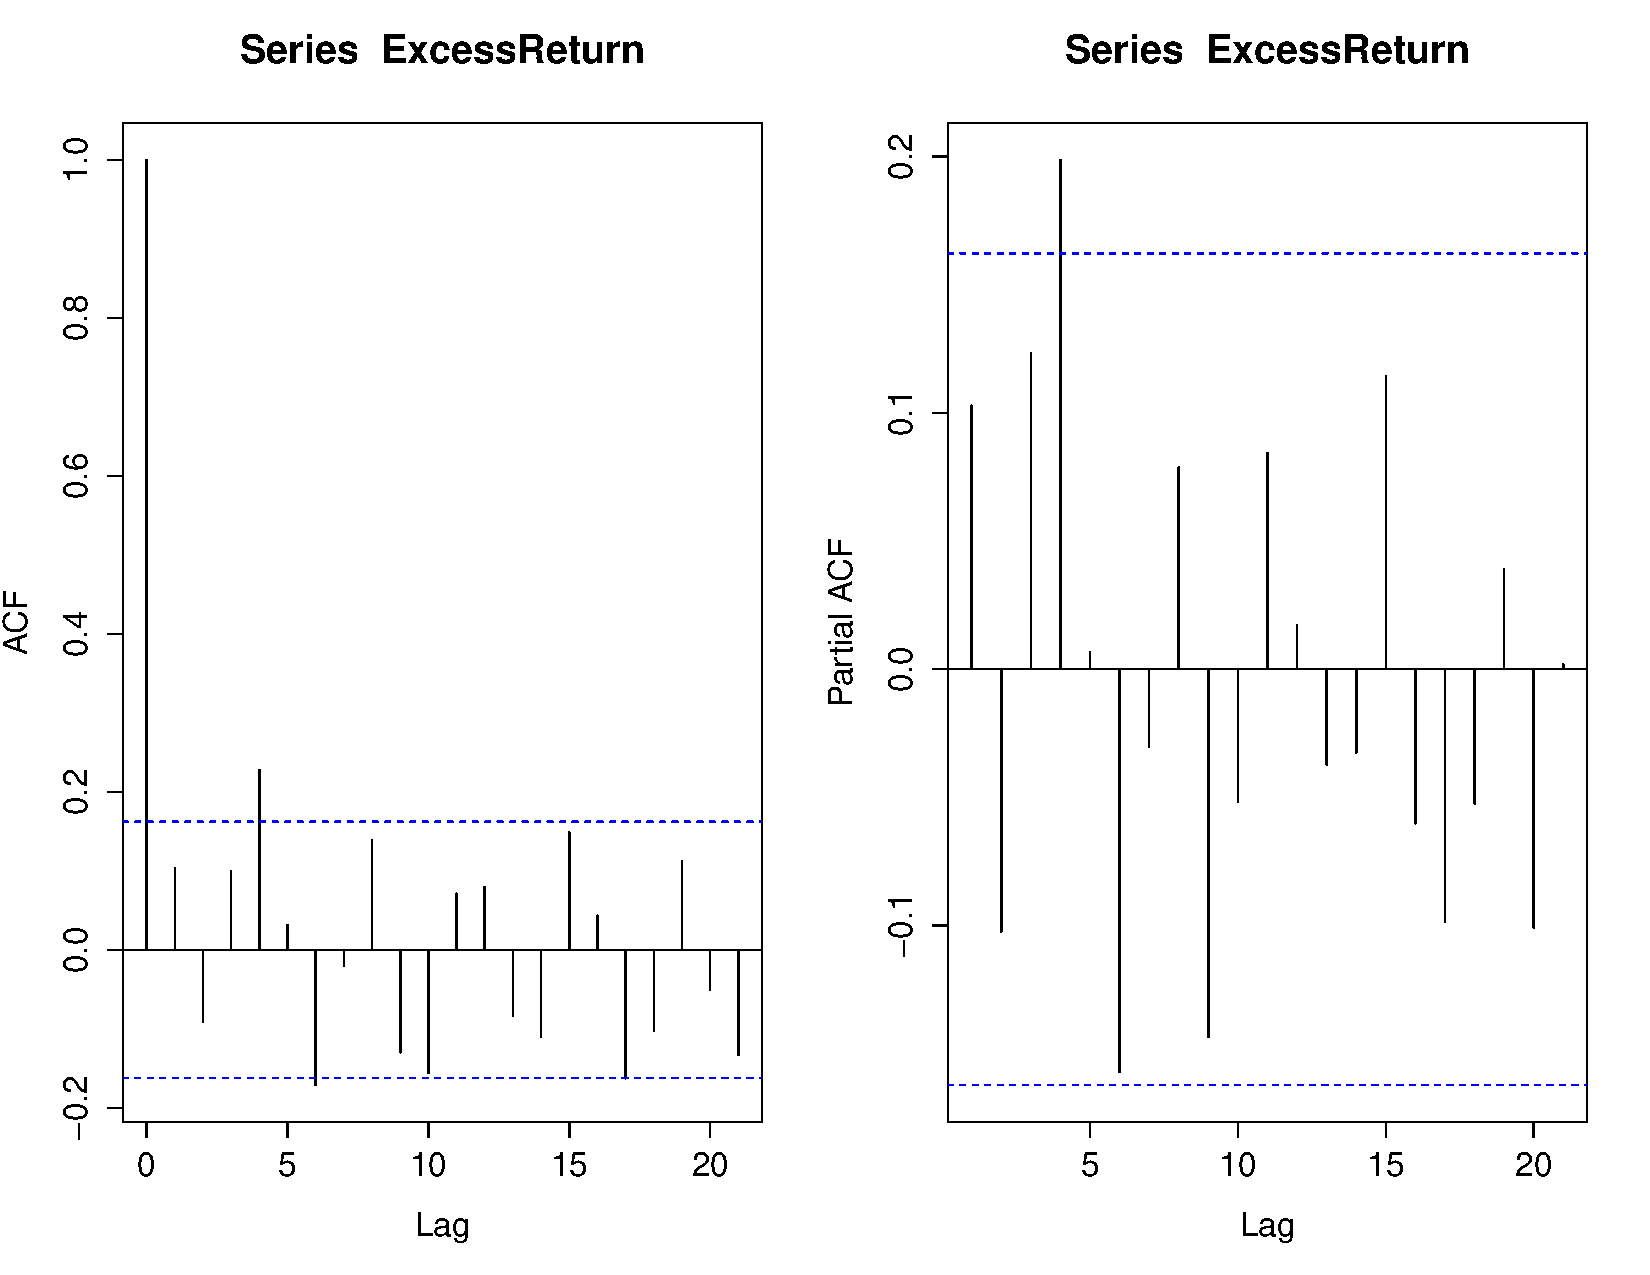
\includegraphics[width=0.8\textwidth]{/Users/zuoyuzhang/desktop/DataAnalysis/2ACF&PACFofTimeSeries.pdf}
    \caption{ACF And PACF Plot Of Monthly Excess Return}
    \label{fig}
	\end{figure}

	\begin{figure}[H]
    \centering
    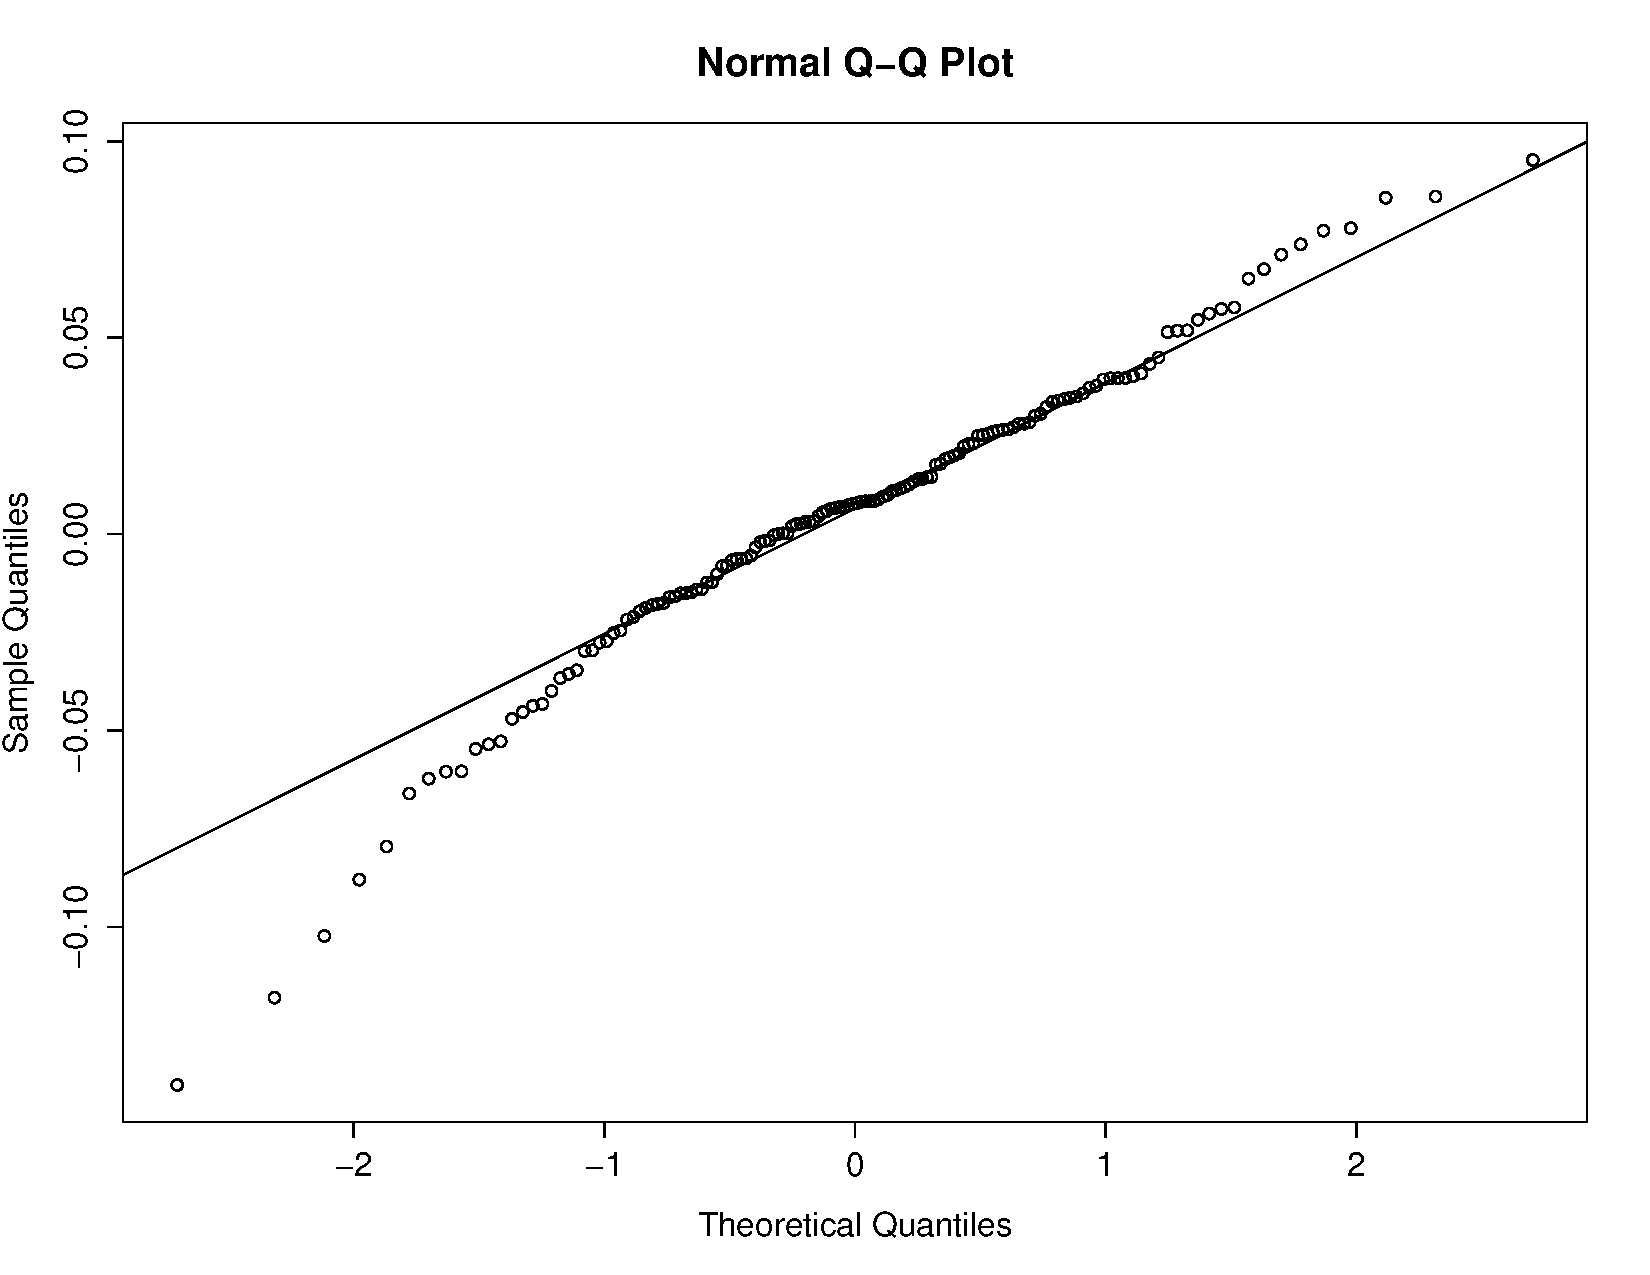
\includegraphics[width=0.8\textwidth]{/Users/zuoyuzhang/desktop/DataAnalysis/ExcessReturnQQplot.pdf}
    \caption{QQ-plot Of Monthly Excess Return}
    \label{fig}
	\end{figure}


	\begin{figure}[H]
    \centering
    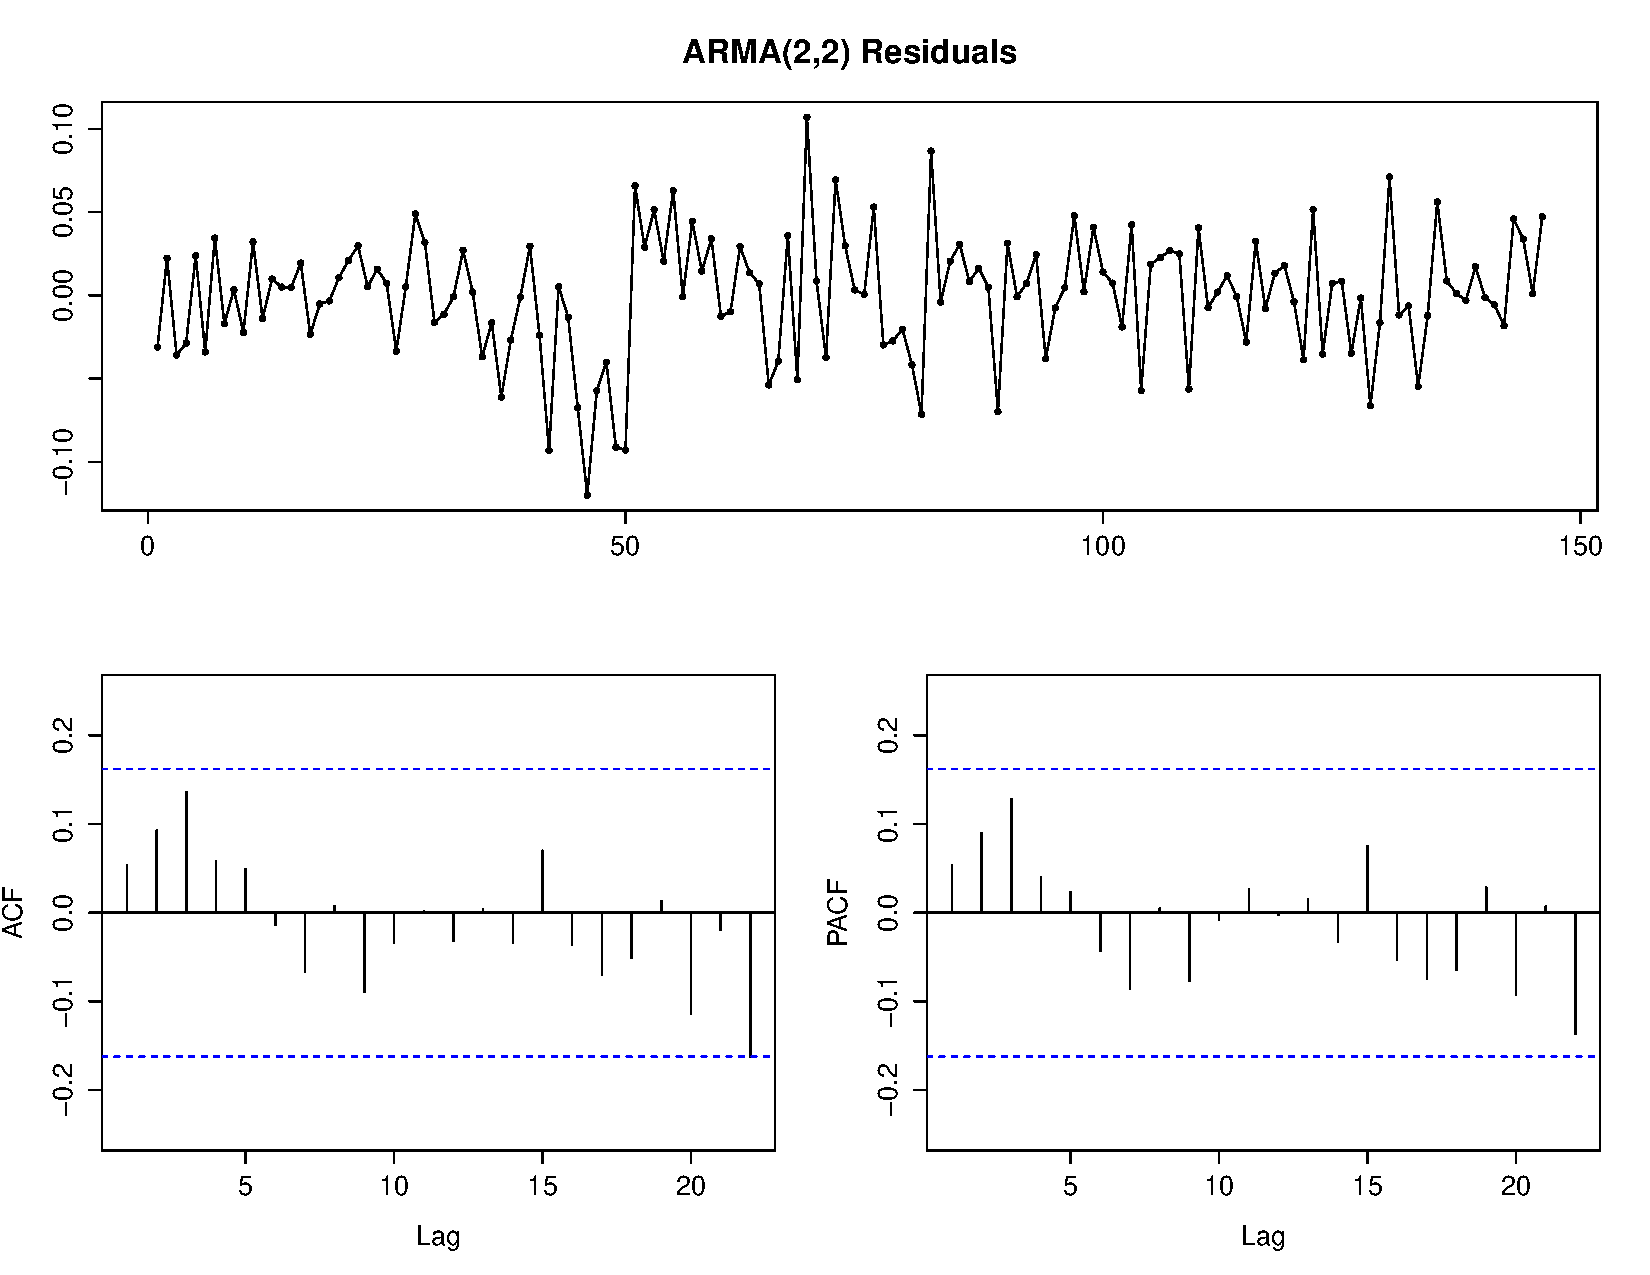
\includegraphics[width=0.8\textwidth]{/Users/zuoyuzhang/desktop/DataAnalysis/Residuals.pdf}
    \caption{ARMA(2,2) Residual Plot And Correlogram}
    \label{fig}
	\end{figure}


	\begin{figure}[H]
    \centering
    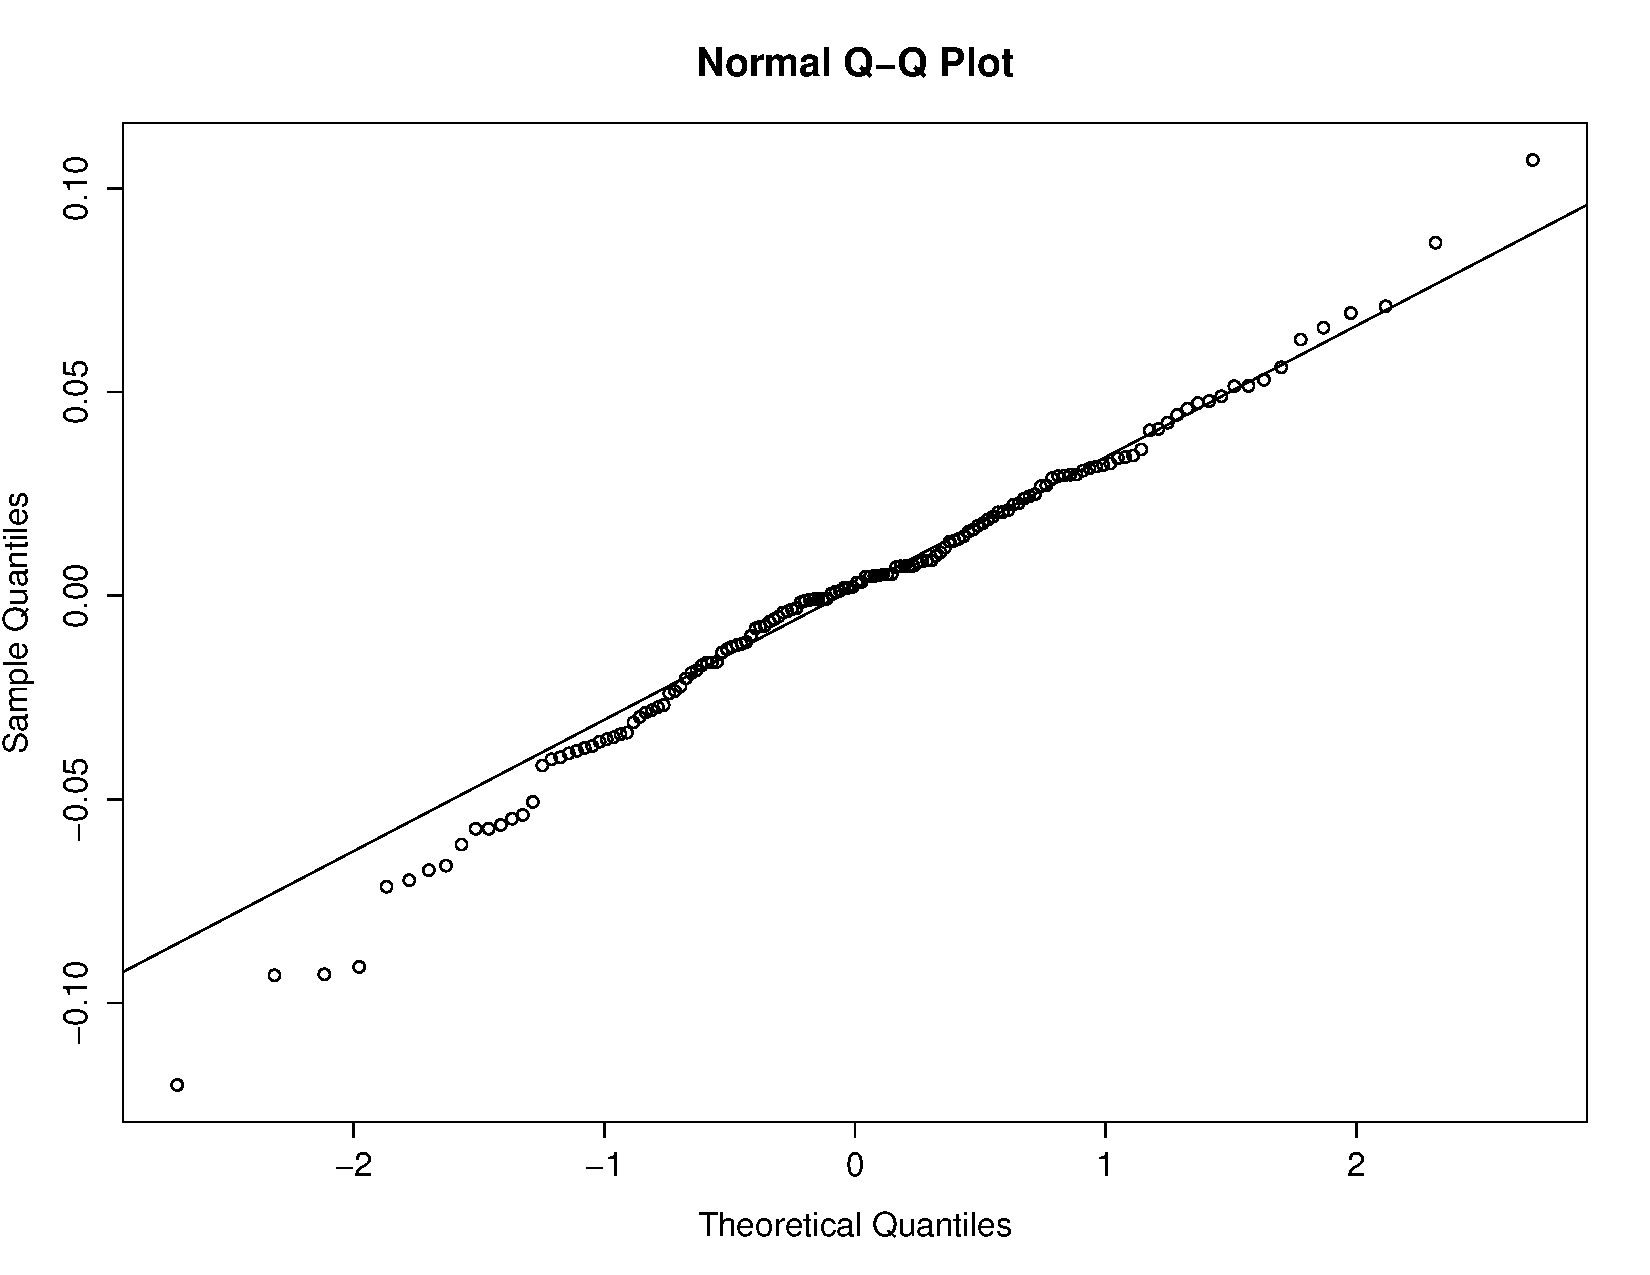
\includegraphics[width=0.8\textwidth]{/Users/zuoyuzhang/desktop/DataAnalysis/ResidualQQplot.pdf}
    \caption{QQ-plot Of ARMA(2,2) Residuals}
    \label{fig}
	\end{figure}	
	
\end{document}